% XeLaTeX document
\documentclass[aspectratio=169, 11pt]{beamer} % для экранов 16:9 оставить

% \documentclass[11pt]{beamer} % для экранов 4:3 оставить

% Редактируем: конфигурация, личные настройки: имя, название предмета и пр. для титульной страницы и метаданных документа здесь
\newcommand{\university}{РГУ нефти и газа (НИУ) имени И.М.Губкина}
\newcommand{\faculty}{кафедра разработки и эксплуатации нефтяных месторождений}
\newcommand{\department}{департамент}
\newcommand{\city}{Москва}
\newcommand{\num}{ № 1}
\newcommand{\docname}{Исследование скважин и пластов. Введение}
\newcommand{\tutorname}{Хабибуллин Р.А.}
\newcommand{\studentname}{студент}
\newcommand{\group}{группы нет}

% Не редактируем: используемые пакеты
% настройка кодировки, шрифтов и русского языка
\usepackage{fontspec}
\usepackage{polyglossia}

% рабочие ссылки в документе
\usepackage{hyperref}

% графика
\usepackage{graphicx}

% качественные листинги кода
\usepackage{minted}
\usepackage{listings}
\usepackage{lstfiracode}

% отключение копирования номеров строк из листинга, работает не во всех просмотрщиках (в Adobe Reader работает)
\usepackage{accsupp}
\newcommand\emptyaccsupp[1]{\BeginAccSupp{ActualText={}}#1\EndAccSupp{}}
\let\theHFancyVerbLine\theFancyVerbLine
\def\theFancyVerbLine{\rmfamily\tiny\emptyaccsupp{\arabic{FancyVerbLine}}}

% библиография
\bibliographystyle{templates/gost-numeric.bbx}
\usepackage{csquotes}
\usepackage[parentracker=true,backend=biber,hyperref=true,bibencoding=utf8,style=numeric-comp,language=auto,autolang=other,citestyle=gost-numeric,defernumbers=true,bibstyle=gost-numeric,sorting=ntvy]{biblatex}

% для заголовков
\usepackage{caption} 

% разное для математики
\usepackage{amsmath, amsfonts, amssymb, amsthm, mathtools}

% водяной знак на документе, см. main.tex
\usepackage[printwatermark]{xwatermark} 

% для презентаций
\usepackage{here}
\usepackage{animate}
\usepackage{bm}

% Не редактируем: параметры используемых пакетов и не только
% настройки polyglossia
\setdefaultlanguage{russian}
\setotherlanguage{english}

% локализация
\graphicspath{ {} }
\addto\captionsrussian{
  \renewcommand{\partname}{Глава}
  \renewcommand{\contentsname}{Содержание}
  \renewcommand{\figurename}{Рисунок}
  \renewcommand{\listingscaption}{Листинг}
}

% основной шрифт документа
\setmainfont{CMU Serif}

% перечень использованных источников
\addbibresource{refs.bib}

% оформление презентации
\usetheme{metropolis}
\usecolortheme{seagull}
\beamertemplatenavigationsymbolsempty

% настройка ссылок и метаданных документа
\hypersetup{unicode=true,colorlinks=true,linkcolor=red,citecolor=green,filecolor=magenta,urlcolor=cyan,        		       
    pdftitle={\docname},   	    
    pdfauthor={\studentname},      
    pdfsubject={\docname},         
    pdfcreator={\studentname}, 	       
    pdfproducer={Overleaf}, 		     
    pdfkeywords={\docname}
}

% настройка подсветки кода и окружения для листингов
\usemintedstyle{colorful}
\newenvironment{code}{\captionsetup{type=listing}}{}

% шрифт для листингов с лигатурами
\setmonofont{FiraCode-Regular.otf}[
    Path = templates/,
    Contextuals=Alternate
]

% путь к каталогу с рисунками
\graphicspath{{fig/}}

% настоящее матожидание
\newcommand{\MExpect}{\mathsf{M}}

% объявили оператор!
\DeclareMathOperator{\sgn}{\mathop{sgn}}

% водяной знак для обозначения статуса документа
\newwatermark[allpages,color=red!5,angle=45,scale=3,xpos=0,ypos=0]{DRAFT}

% настройка метаданных документа
\institute[\university]{\university \\ \faculty}
\title[\docname]{\docname}
\author[\tutorname]{\small Преподаватель: \tutorname}
\date{\the\year} 

\makeatletter
\setbeamertemplate{title page}{
  \begin{minipage}[b][\paperheight]{\textwidth}
    \centering
    \ifx\insertinstitute\@empty\else\usebeamertemplate*{institute}\fi
    \vfill
    \ifx\inserttitle\@empty\else\usebeamertemplate*{title}\fi
    \vfill
    \usebeamertemplate*{title separator}
    \ifx\beamer@shortauthor\@empty\else\usebeamertemplate*{author}\fi
    \ifx\insertdate\@empty\else\usebeamertemplate*{date}\fi
    \vfill
    \vspace*{1mm}
  \end{minipage}
}

\setbeamertemplate{title}{
  \vspace{0.5cm}
  \inserttitle
  \par
  \vspace*{0.5em}
}

\setbeamertemplate{date}{
  \vspace{0.5cm}
  \city \\
  \insertdate
  \par
  \vspace*{0.5em}
}
\makeatother
\setbeamerfont{institute}{size=\footnotesize}
\setbeamerfont{date}{size=\footnotesize}


\begin{document}

% Редактируем: всё остальное: вступление, др. этапы, заключение, приложение
\begin{frame}
    \titlepage
\end{frame}

% ---------------------------------------------------------------------------------------------
\begin{frame}{Содержание курса}
\begin{enumerate}
    \item Введение в дисциплину. Зачем надо проводить исследования?
    \item Исследования и замеры в работающих скважинах. Построение моделей работающих скважин. Барометрия, термометрия, дебитометрия.
    \item Исследования пласта и призабойной зоны. Гидродинамические исследования. Построение простых моделей.
    \item ГДИС. Интерпретация исследований.
    \item Исследования пласта и скважин. Прокси модели пласта. Оптимизация работы скважин.
\end{enumerate}
Курс состоит из набора задач.
\end{frame}

% ---------------------------------------------------------------------------------------------
\begin{frame}{Расписание 2020 года}
Расписание отличается от прошлых лет.
\begin{itemize}
    \item 6 семинаров очно -- по 3 пары каждую неделю 
    \item Лекции онлайн (9 лекций) на \href{edu.gubkin.ru}{edu.gubkin.ru} 
\end{itemize}

Схема работы в течении семестра:
\begin{itemize}
    \item На сайте \href{edu.gubkin.ru}{edu.gubkin.ru} лекции и материалы для решения задач, а также задания
    \item Семинары -- разбор решения задач. Будет 5 блоков задач. Желательны компьютеры на семинарах. 
    \item На сайте \href{edu.gubkin.ru}{edu.gubkin.ru} оценки и отчеты о выполнении заданий
\end{itemize}

\end{frame}

% ---------------------------------------------------------------------------------------------
\begin{frame}{Курс 2020 года. Баллы}
Цель курса - научиться решать задачи связанные с исследованием скважин и пластов с использованием различных инструментов для проведения расчетов. 

Способы набрать баллы:
\begin{itemize}
    \item решение задач (от 1 до 10 баллов за задачу) -- основной способ;
    \item работа с материалами на сайте, подготовка материалов, полезные посты на форуме (от 1 до 5 баллов за активность);
    \item работа на семинарах, доклады по проведенной работе (от 1 до 3 баллов);    
\end{itemize}

\end{frame}

\begin{frame}{Дополнительные слайды}
Дальше пойдут слайды с примерами подготовки презентации, которые потом надо будет удалить 
\end{frame}


\begin{frame}{Заполнение шаблона}
\begin{itemize}
    \item Изменить \textbf{config.tex}: имя студента, название предмета и пр. параметры указаны именно там
    \item Заполнить \textbf{content.tex} - файл, который будет содержать весь текст презентации.
    \item Добавить используемую литературу (если есть) в \textbf{refs.bib}. Для удобного поиска источников можно воспользоваться Google Books. Использованные источники можно указывать с помощью команды \textbf{\\cite\{name\_of\_ref\}}
\end{itemize}
Далее представлены различные примеры.
\end{frame}

\begin{frame}{Обычный слайд текста}
Текст сам центрируется по высоте слайда. Центрирование по горизонтали 
\end{frame}


\begin{frame}{Список}
\begin{itemize}
	\item Элемент списка
	\begin{itemize}
		\item Элемент вложенного списка
	\end{itemize}
	\item Элемент списка
	\begin{enumerate}
		\item Элементы
		\item нумерованного
		\item списка
	\end{enumerate}
\end{itemize}
\end{frame}

\begin{frame}{Блоки}
\begin{exampleblock}{Заголовок блока}
	Текст блока примера. Кстати, ссылка \cite{kingma2014adam}
\end{exampleblock}

\begin{alertblock}{}
	Текст блока предупреждения 
\end{alertblock}

\end{frame}

\begin{frame}{Рисунок}
\begin{figure}[H]
	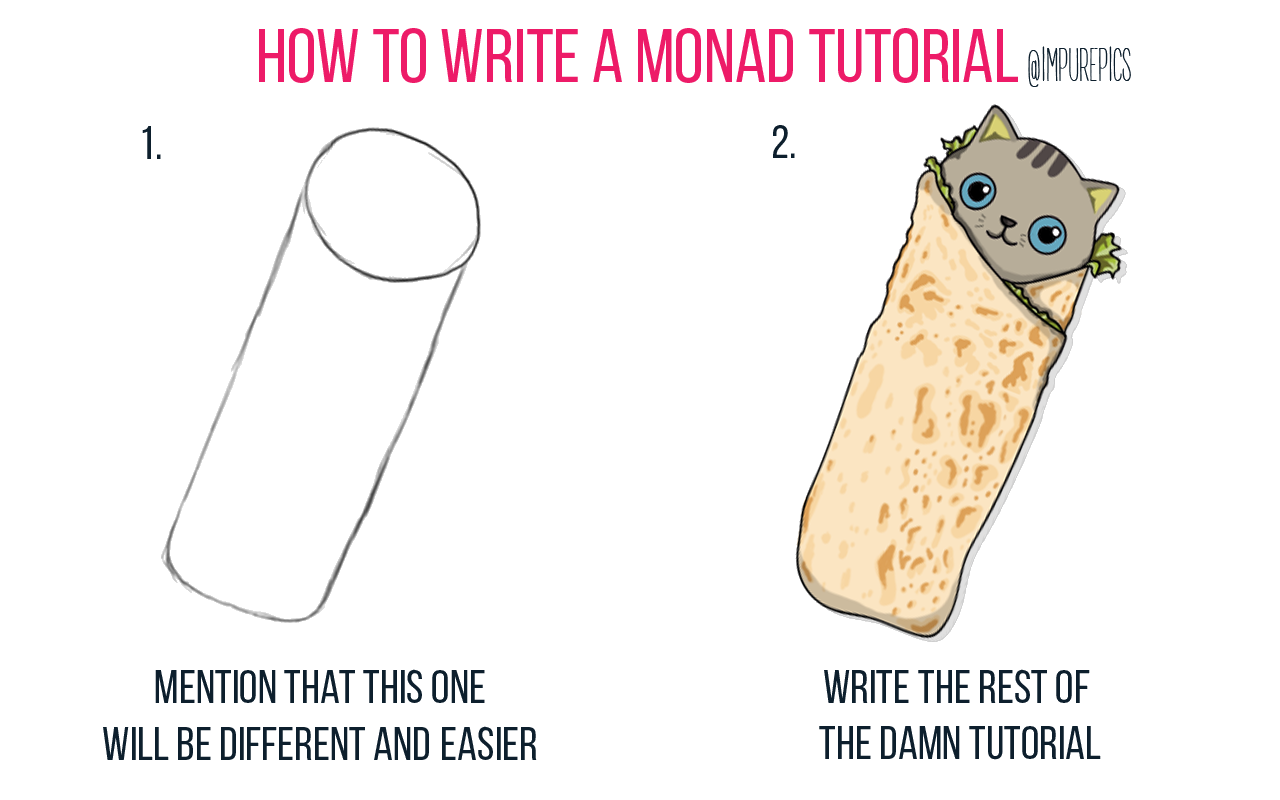
\includegraphics[width=0.5\textwidth]{fig/sample.png}
	\label{fig:sample}
	\caption{Подпись}
\end{figure}
\center{\url{https://impurepics.com/}}
\end{frame}

\begin{frame}{Листинг}
\begin{code}
    \inputminted[breaklines=true, xleftmargin=1em,linenos, frame=single, framesep=10pt, firstline=1, lastline=7]{haskell}{listings/haskell_code.hs}
    \caption{Да, это опять функциональный код.}
\end{code}
\end{frame}

\begin{frame}{Формулы, сложна}
Спектр (спектральная плотность) $\Phi(f)$ в общем случае представляет собой комплексную функцию: $$\Phi(f)=|\Phi(f)|*e^{i\psi(f)}$$
Модуль этой функции $|\Phi(f)|$ называют спектром амплитуд, а зависимость $\psi(f)$ — спектром фаз.
\end{frame}

\begin{frame}[fragile]{Разбиваем слайд}
Раз.
\pause
Два.
\pause
Ну вы поняли.
\end{frame}

\begin{frame}{Анимация?}
\begin{figure}
\begin{tabular}{c}
Но нужен Adobe Reader. Или что-то другое хорошее. \\
  \animategraphics[loop,controls,width=0.9\textwidth]{1}{fig/sgd/descent-}{0}{7}
\end{tabular}
\end{figure}
\end{frame}

\begin{frame}{Перечень использованных источников}
\printbibliography[title=Этот цвет тоже можно поменять.]
\end{frame}


% Не редактируем: Страница библиографии (формируется автоматически из книжек, указанных в refs.bib и пометок \cite{имя_источника} в тексте)
\include{templates/bib-page}

\end{document}
